\documentclass[twoside]{article}
\setlength{\oddsidemargin}{0.25 in}
\setlength{\evensidemargin}{-0.25 in}
\setlength{\topmargin}{-0.6 in}
\setlength{\textwidth}{6.5 in}
\setlength{\textheight}{8.5 in}
\setlength{\headsep}{0.75 in}
\setlength{\parindent}{0 in}
\setlength{\parskip}{0.1 in}
\newcommand{\eqdef}{:\mathrel{\mathop=}}
\newcommand{\norm}[1]{\left\lVert #1 \right\rVert}

%
% ADD PACKAGES here:
%

\usepackage{amsmath,amsfonts,graphicx}

%
% The following commands set up the lecnum (lecture number)
% counter and make various numbering schemes work relative
% to the lecture number.
%
\newcounter{lecnum}
\renewcommand{\thepage}{\thelecnum-\arabic{page}}
\renewcommand{\thesection}{\thelecnum.\arabic{section}}
\renewcommand{\theequation}{\thelecnum.\arabic{equation}}
\renewcommand{\thefigure}{\thelecnum.\arabic{figure}}
\renewcommand{\thetable}{\thelecnum.\arabic{table}}

%
% The following macro is used to generate the header.
%
\newcommand{\lecture}[4]{
   \pagestyle{myheadings}
   \thispagestyle{plain}
   \newpage
   \setcounter{lecnum}{#1}
   \setcounter{page}{1}
   \noindent
   \begin{center}
   \framebox{
      \vbox{\vspace{2mm}
    \hbox to 6.28in { {\bf Advanced Machine Learning
	\hfill Fall 2020} }
       \vspace{4mm}
       \hbox to 6.28in { {\Large \hfill Lecture #1: #2  \hfill} }
       \vspace{2mm}
       \hbox to 6.28in { {\it  #3 \hfill  #4} }
      \vspace{2mm}}
   }
   \end{center}
   \markboth{Lecture #1: #2}{Lecture #1: #2}

   {\bf Note}: {\it LaTeX template courtesy of UC Berkeley EECS dept.}

   {\bf Disclaimer}: {\it These notes are adapted from ETH's Advanced Machine Learning Course, EPFL's CS433 Course, Stanford's CS231N Course and "Neural Networks and Deep Learning" book.}
   \vspace*{4mm}
}
%
% Convention for citations is authors' initials followed by the year.
% For example, to cite a paper by Leighton and Maggs you would type
% \cite{LM89}, and to cite a paper by Strassen you would type \cite{S69}.
% (To avoid bibliography problems, for now we redefine the \cite command.)
% Also commands that create a suitable format for the reference list.
\renewcommand{\cite}[1]{[#1]}
\def\beginrefs{\begin{list}%
        {[\arabic{equation}]}{\usecounter{equation}
         \setlength{\leftmargin}{2.0truecm}\setlength{\labelsep}{0.4truecm}%
         \setlength{\labelwidth}{1.6truecm}}}
\def\endrefs{\end{list}}
\def\bibentry#1{\item[\hbox{[#1]}]}

%Use this command for a figure; it puts a figure in wherever you want it.
%usage: \fig{NUMBER}{SPACE-IN-INCHES}{CAPTION}
\newcommand{\fig}[3]{
			\vspace{#2}
			\begin{center}
			Figure \thelecnum.#1:~#3
			\end{center}
	}
% Use these for theorems, lemmas, proofs, etc.
\newtheorem{theorem}{Theorem}[lecnum]
\newtheorem{lemma}[theorem]{Lemma}
\newtheorem{proposition}[theorem]{Proposition}
\newtheorem{claim}[theorem]{Claim}
\newtheorem{corollary}[theorem]{Corollary}
\newtheorem{definition}[theorem]{Definition}
\newenvironment{proof}{{\bf Proof:}}{\hfill\rule{2mm}{2mm}}

% **** IF YOU WANT TO DEFINE ADDITIONAL MACROS FOR YOURSELF, PUT THEM HERE:

\newcommand\E{\mathbb{E}}

\begin{document}
%FILL IN THE RIGHT INFO.
%\lecture{**LECTURE-NUMBER**}{**DATE**}{**LECTURER**}{**SCRIBE**}
\lecture{10}{Deep Learning}{}{}
%\footnotetext{These notes are partially based on those of Nigel Mansell.}

% **** YOUR NOTES GO HERE:

% Some general latex examples and examples making use of the
% macros follow.  
%**** IN GENERAL, BE BRIEF. LONG SCRIBE NOTES, NO MATTER HOW WELL WRITTEN,
%**** ARE NEVER READ BY ANYBODY.


\section{Neural Networks} % Don't be this informal in your notes!
Let us look at the structure of a neural network. It is shown
in Figure 10.1. This is a neural net with one input layer of size
$\mathbf{D}$, $\mathbf{L}$ hidden layers of size $\mathbf{K}$, and one output layer. It is
a feedfoward network: the computation performed by the
network starts with the input from the left and flows to the
right. There is no feedback loop.
As always, we assume that our input is a $\mathbf{D}$-dimensional
vector. We see that there is a node drawn in Figure 1 for
each of the $D$ components of $x$. We denote these nodes by
$x^{(0)}_{i}$
, where the superscript $(0)$ specifies that this is the input
layer.
\begin{figure}[h]
\centering

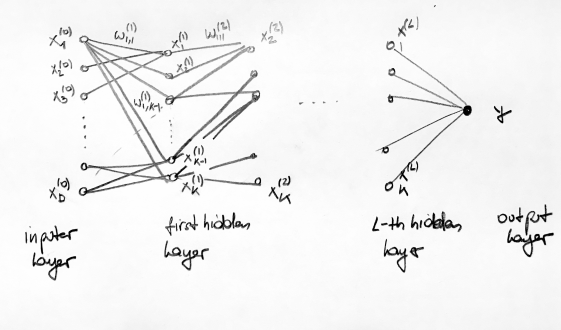
\includegraphics[width=0.5\textwidth]{img/nn.png}
\caption{A neural network with one input layer, L hidden
layers, and one output layer.}
\end{figure}
 
 Let us assume that there are $\mathbf{K}$ nodes in each hidden layer, where $K$ is a hyper-parameter. Each node in the hidden layer $l, \; l = 1, \ldots , L$, is connected
to all the nodes in the previous layer via a weighted edge.
We denote the edge from node $i$ in layer $l - 1$ to the node
$j$ in layer $l$ by $w^{(l)}_{i,j} $. The super-script $(l)$ indicates that these
are the weights of edges that lead to layer $l$. The output at the node $j$ in layer $l$ is denoted by $x^{(l)}_{j}$ and it is given by:
$$ x^{(l)}_{j}  = \phi \Big( \sum_{i} w_{i,j}^{(l)} x_{i}^{(l-1)} + b_{j}^{(l)} \Big) $$

In simple words, in order to compute the output we first compute
the weighted sum of the inputs and then apply a function $\phi$
to this sum.
\newpage
A few remarks:

\begin{itemize}
    \item The constant term $b^{(l)}_{j}$ is called the \textbf{bias term} and is a parameter like any of the weights $w^{(l)}_{i,j}$ . The learning part will consist of choosing all these parameters appropriately for the task.
    \item The function $\phi$
is called the \textbf{activation function}. It is crucial that this function is \textbf{non-linear}.\\ Why is this?
Assume not, then the whole neural-net would just be a highly
factorized linear function of the input data and there would
be no gain compared to standard linear regression/classification. 
\end{itemize}
\subsection{Representation Power}

How “powerful” are neural nets? More precisely, what functions $f(x)$ can they represent, or better, what functions can they approximate? Before we get into our heuristic argument let us state the
main theorem of the paper by Barron: “Universal approximation bounds for superpositions of a sigmoidal function”. This gives you a
flavor of what kind of results can be proved.

\begin{lemma}
Let $f: \mathbb{R}^{D} \rightarrow \mathbb{R}$ be a function such that $$\int_{\mathbb{R}^{D}} |w||\Tilde{f}(w)|dw \leq C$$
where 
$$\Tilde{f}(w) = \int_{\mathbb{R}^{D}} f(x) e^{-jw^T x}dx$$
is the Fourier transform of $f(x)$\\
\\Then for all $n \geq 1 $, there exists a function $f_{n}$ of the form
$$f_{n}(x) = \sum_{j=1}^{n}c_{j}\phi(x^T w_{j} + b_{j}) + c_{0}$$
i.e., a function that is representable by a NN with one
hidden layer with n nodes and “sigmoid-like” activation
functions so that
$$\int_{|x| \leq r}(f(x) - f_{n}(x))^2dx \leq \dfrac{(2Cr)^2}{n}$$
\end{lemma}
Let's discuss this result:
\begin{itemize}
    \item First note that the condition on the Fourier
transform is a “smoothness condition.” E.g., functions so
that $\int_{\mathbb{R}^{D}} |w||\Tilde{f}(w)|dw \leq \infty$ can be shown to be continuously
differentiable.
\item Second note that the lemma only guarantees a good approximation in a \textbf{bounded domain}. The larger the domain, the more nodes we need in order to approximate a function to the same level (see the term $r^2$, where $r$ is the radius of the ball where we want the approximation to be good, in the upper bound).
\item Third, this is an approximation “in average”, more precisely in $\mathbb{L}_{2}$-norm. 
\item Fourth, the approximation $f_{n}$ with $n$ terms corresponds exactly to our model of a neural net with one hidden layer containing $n$ nodes and sigmoids as activation functions.
\item Fifth, the theorem applies to all activation functions that are
“sigmoid-like,” i.e., all activation functions whose left limit
is $0$, whose right limit is $1$, and that are sufficiently smooth.
\end{itemize}
In simple words, the lemma says that a sufficiently “smooth” function can be approximated by a neural net with one hidden
layer and the approximation error goes down like one over
the number of nodes in the hidden layer. Note that this is a
very fast convergence.
\subsection{Approximation in Average}
We start with a scalar function $f(x): \mathbb{R} \rightarrow \mathbb{R}$ on a bounded domain. Recall that if this function is continuous then it is Riemann integrable, i.e., it can be approximated arbitrarily closely
by “upper” and “lower” sums of rectangles, see Figure 10.2. Of course, we might need a lot of such rectangles to approximate
the area with an error of at most $\epsilon$, but for every $\epsilon > 0$ we
can find such an approximation. 

\begin{figure}[h]
\centering

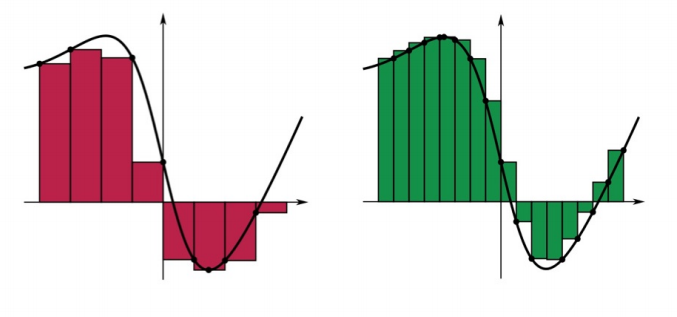
\includegraphics[width=0.5\textwidth]{img/riemann.png}
\caption{A lower and an upper Riemann sum.}
\end{figure}

We will now show that if we do not limit the weights, then
with two hidden nodes (of a neural network with one hidden
layer) we can construct a function which is arbitrarily close
to a given rectangle. But since, as we have just seen, a finite number of rectangles suffices to approximate a bounded
continuous function arbitrarily closely, it follows that with a
finite number of hidden nodes of a neural network with one
hidden layer we can approximate any such function arbitrarily closely.\\ \\
Let $\phi(x) = \dfrac{1}{1+e^{-x}}$ be the sigmoid function. Consider the function $f(x) = \phi(w(x - b))$, where $w$ is the
weight of a particular edge and $-wb$ is the bias term. \\If we want to create a rectangle that jumps from
$0$ to $1$ at $x = a$ and jumps back to $0$ at $x = b$, $a < b$, then we can accomplish this by taking
$$\phi(w(x - a)) - \phi(w(x - b))$$
and taking $w$ very large (see Figure 10.3).


\begin{figure}[h]
\centering

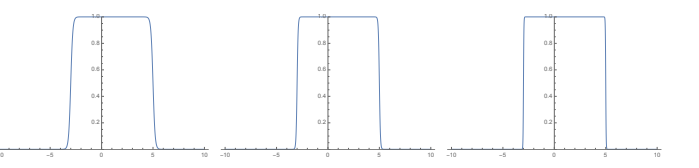
\includegraphics[width=0.5\textwidth]{img/riemann_nn.png}
\caption{An approximate rectangle of the form $\phi(w(x -
a))-\phi(w(x-b))$ with $w = 10$, $20$, and $50$, respectively.}
\end{figure}

Note that these "rectangles"  have a very simple representation in
form of a neural network. This is shown in Figure 10.4. There is
one input node which contains the value x. This value is multiplied by some large weight (in the figure it is 50) and
it is then forwarded to the two hidden nodes. One of these
hidden nodes has a bias of 150 the other one has a bias
of -250, so that the sums at these two hidden nodes are
$50(x + 3)$ and $50(x - 5)$, respectively. Each node applies the
sigmoid function and forwards the result to the output layer.
The edge from the top hidden node to the output has weight
1 and the one from the bottom hidden node to the output
has weight -1. The output node adds the two inputs. The
result is $\phi(50(x+ 3))-\phi(50(x-5))$, which is approximately
a unit-height rectangle from -3 to 5.

\begin{figure}[h]
\centering
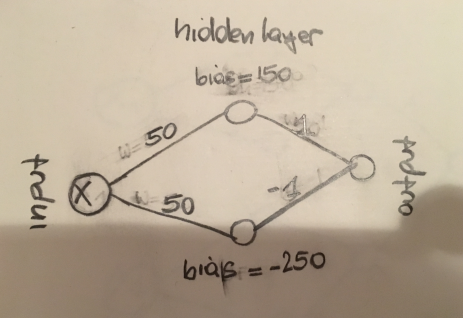
\includegraphics[width=0.5\textwidth]{img/nn_rect.png}
\caption{A simple NN implementation of a unit-height rectangle from -3 to 5}
\end{figure}


It is hopefully clear at this point why any continuous function
on a bounded domain can be approximated via a neural
network with one hidden layer. Let us summarize in telegram
style: Take the function. Approximate it in the Riemann sense. Approximate each of the rectangles in the Riemann
sum by means of two nodes in the hidden layer of a neural
net. Compute the sum (with appropriate sign) of all the
hidden layers at the output node. If we are using a Riemann
sum with $\mathbf{K}$ rectangles we get therefore a neural network
approximation with one hidden layer containing $\mathbf{2K}$ nodes.
\newpage

\subsection{Activation Functions}
There are many activation functions that are being used in
practice. Let us list here some of them and briefly discuss
their merits.

\paragraph{Sigmoid}
We start with the sigmoid $\phi(x)$, which we have encountered
already several times. Just to summarize, it is defined by:
$$\phi(x) = \dfrac{1}{1+e^{-x}}$$
and a plot is shown in Figure 10.5. Note that the sigmoid is always positive (not really an issue) and that it is bounded. \\ Further, for $|x|$ large, $ \phi'(x)  \approx 0$. This can cause the gradient to become very small (which is known as the “\textbf{vanishing
gradient problem}”), sometimes making learning slow.


\begin{figure}[h]
\centering
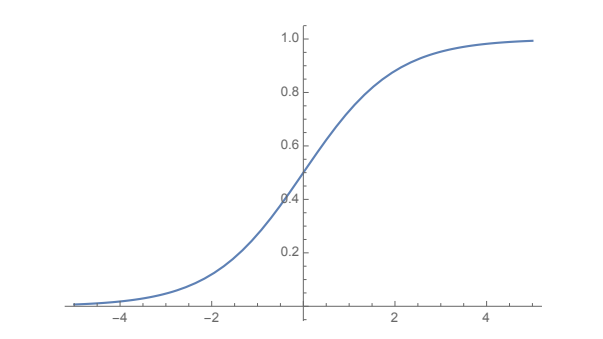
\includegraphics[width=0.43\textwidth]{img/sigmoid.png}
\caption{The sigmoid function $\phi(x)$.}
\end{figure}

\paragraph{Tanh}
Very much related to the sigmoid is $tanh(x)$. It is defined by
$$tanh(x) = \dfrac{e^x - e^{-x}}{e^x + e^{-x}} = 2\phi(2x) -1$$
and a plot is shown in Figure 10.6. 

\begin{figure}[h]
\centering
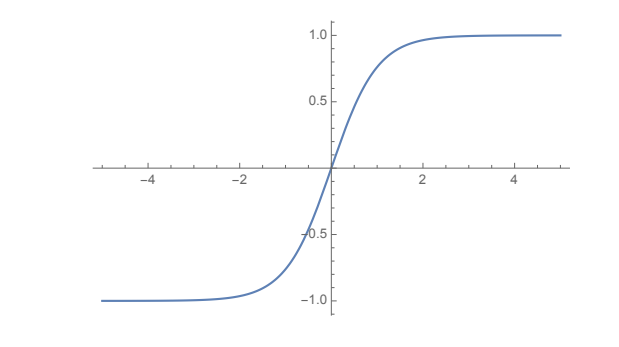
\includegraphics[width=0.43\textwidth]{img/tanh.png}
\caption{The function $\tanh(x)$.}
\end{figure}

Note that $tanh(x)$ is “balanced” (positive and negative) and that it is bounded. But
it has the same problem as the sigmoid function, namely for
$|x|$ large, $tanh'(x) \approx 0$. As mentioned before, this can cause the
gradient to become very small, sometimes making learning slow.

\paragraph{Rectified linear Unit – ReLU}
Very popular is the rectified linear unit (ReLU) , which is defined by
$$(x)_{+} = max\{0,x\}$$
and a plot is shown in Figure 10.7.

\begin{figure}[h]
\centering
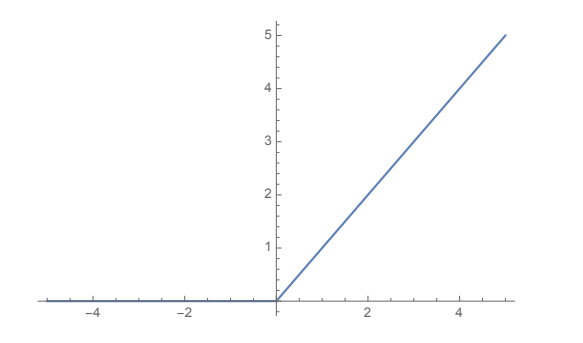
\includegraphics[width=0.43\textwidth]{img/relu.png}
\caption{The ReLU $(x)_{+}$.}
\end{figure}

Note that the ReLU is always positive and that it is unbounded. One nice property
of the ReLU is that its derivative is $1$ (and does not vanish)
for positive values of $x$ (it has $0$ derivative for negative values
of $x$ though).

\paragraph{Leaky ReLU}
In order to solve the $0$-derivative problem of the ReLU (for
negative values of $x$) one can add a very small slope $\alpha$ in
the negative part. This gives rise to the leaky rectified linear
unit (LReLU), which is defined by

$$f(x) = max\{ \alpha x, x\}$$
and a plot is shown in Figure 10.8. The constant $\alpha$ is of course
a hyper-parameter that can be optimized.

\begin{figure}[h]
\centering
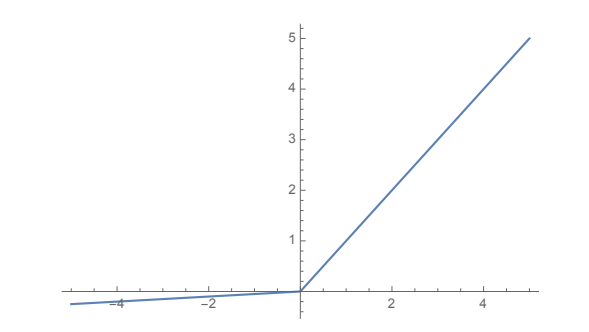
\includegraphics[width=0.43\textwidth]{img/lrelu.png}
\caption{LReLU with $\alpha = 0.05$.}
\end{figure}

\newpage

\subsection{Compact Description of Output}
Let us start by writing down the output as a function of the input explicitly in compact form. It is natural and convenient to describe the function that is implemented by each layer of the network separately at first. The overall function is then
the composition of these functions. \\ \\
Let $\mathbf{W}^{(l)}$ denote the weight matrix that connects layer $l  - 1$
to layer $l$. The matrix $W^{(1)}$ is of dimension $D \times K$, the
matrices $W^{(l)}$
, $2 \leq l \leq L$, are of dimension $K \times K$, and the
matrix $W^{(L+1)}$ is of dimension $K \times 1$. The entries of each
matrix are given by

$$W^{(l)}_{i,j} = w^{(l)}_{i,j} $$

where we recall that $ w^{(l)}_{i,j}$ is the weight on the edge that connects node $i$ on layer $l - 1$ to node $j$ on layer $l$.\\ 
Further, let us introduce the bias vectors 
$\mathbf{b}^{(l)}$, $1 \leq l \leq L+1$,
that collect all the bias terms. All these vectors are of length
$K$, except the term $b^{(L+1)}$, that is a scalar. \\ \\
With this notation we can describe the function that is implemented by each layer in the form: 
$$x^{(l)} = f^{(l)}(x^{(l-1)}) = \phi((W^{(l)})^T  x^{(l-1)} + b^{(l)})$$

where the (generic) activation function is applied point-wise to the vector.
The overall function $y = f(x
^{(0)})$ can then be written in terms
of these functions as the composition:
$$f(x^{(0)}) = f^{(L+1)} \circ \ldots \circ f^{(2)} \circ f^{(1)}(x^{(0)}).$$

\subsection{The Backpropagation Algorithm}
The cost function can be written as:

$$\mathcal{L} = \dfrac{1}{N} \sum_{i=1}^{N} (y_{i} -f^{(L+1)} \circ \ldots \circ f^{(2)} \circ f^{(1)}(x_{i}))^2$$

Note that this cost function is a function of all weight matrices and bias vectors and that it is a composition of all the functions describing the transformation at each layer.\\
Note also that the specific form of the loss does not really matter for the workings of the back propagation algorithm that we now discuss. Just to be
specific we stick to the square loss. Only the initialization of the back recursion changes if we pick a different loss function.

In SGD we compute the gradient of this function with respect to one single sample. Therefore, we start with the function:

$$\mathcal{L}_{n} =  (y_{n} -f^{(L+1)} \circ \ldots \circ f^{(2)} \circ f^{(1)}(x_{n}))^2$$
Recall that our aim is to compute:
\begin{equation*}
\begin{aligned}
   & \dfrac{\partial \mathcal{L}_{n} }{\partial  w^{(l)}_{i,j} } , \; l=1,\ldots,L+1 \\
   & \dfrac{\partial \mathcal{L}_{n} }{\partial  b^{(l)}_{j} } , \; l=1,\ldots,L+1
  \end{aligned}
\end{equation*}

It will be convenient to first compute two preliminary quantities. The desired derivatives are then easily expressed in
terms of those quantities.
Let:

$$z^{(l)} = (W^{(l)})^T  x^{(l-1)} + b^{(l)}$$

where $x^{(0)} = x_{n}$ and $x^{(l)} = \phi(z^{(l)})$. In simple words, $z^{(l)}$
is the input at the $l$-th layer before applying the activation function. These quantities are easy to compute by a \textbf{forward pass} in the network. \\More precisely, start with $x^{(0)} = x_{n}$ and
then apply this recursion for $l = 1, \ldots, L + 1$, first always computing $z^{(l)}$ and then computing $x^{(l)} = \phi(z^{(l)})$.\\ \\
Further, let
$$\delta_{j} = \dfrac{\partial \mathcal{L}_{n} }{\partial z^{(l)}_{j}}$$

Let $\delta ^{(l)}$ be the corresponding vector at level $l$. Whereas the
quantities $z^{(l)}$ were easily computed by a forward pass, the quantities $\delta^{(l)}$
are easily computed by a \textbf{backwards pass}:
\begin{equation*}
\begin{aligned}
   & \delta^{(l)}_{j} =  \dfrac{\partial \mathcal{L}_{n} }{\partial z^{(l)}_{j}} =
   \sum_{k=1}^{K} \dfrac{\partial \mathcal{L}_{n} }{\partial z^{(l+1)}_{k}} \dfrac{\partial z^{(l+1)}_{k}}{\partial z^{(l)}_{j}} 
   \\
   & = \sum_{k=1}^{K} \delta_{k}^{(l+1)} W^{(l+1)}_{j,k} \phi'(z_{j}^{(l)})
  \end{aligned}
\end{equation*}
The sum comes from the fact the loss $\mathcal{L}_{n}$ at the layer $l+1$ is the sum of the losses evaluated at each of the neurons ($z_{k}$) in that layer, then we applied the chain rule. In vector form, we can write this as:
$$\delta^{(l)} = (W^{(l+1)}\delta^{(l+1)}) \odot \phi'(z^{(l)})$$

where $\odot$ denotes the Hadamard product. Now that we both have $z^{(l)}$ and $\delta^{(l)}$ let us get back to our initial goal:
$$\dfrac{\partial \mathcal{L}_{n} }{\partial w^{(l)}_{i,j}} = \sum_{k=1}^{K} \dfrac{\partial \mathcal{L}_{n} }{\partial z^{(l)}_{k}}  \dfrac{\partial z^{(l)}_{k}}{\partial w^{(l)}_{i,j}} = 
\overbrace{\dfrac{\partial \mathcal{L}_{n} }{\partial z^{(l)}_{j}}}^\text{$\delta^{(l)}_{j}$}  \overbrace{\dfrac{\partial z^{(l)}_{j}}{\partial w^{(l)}_{i,j}}}^\text{$x_{i}^{(l-1)}$} =\delta^{(l)}_{j}  x_{i}^{(l-1)}$$

Why could we drop the sum in the above expression? When we change the weight $w^{(l)}_{i,j}$ then it only changes the sum $z^{(l)}_{j}$.
All other sums at level $l$ stay unchanged.
\\In a similar manner,
$$\dfrac{\partial \mathcal{L}_{n} }{\partial b^{(l)}_{j}} = \sum_{k=1}^{K} \dfrac{\partial \mathcal{L}_{n} }{\partial z^{(l)}_{k}}  \dfrac{\partial z^{(l)}_{k}}{\partial b^{(l)}_{j}} = 
\overbrace{\dfrac{\partial \mathcal{L}_{n} }{\partial z^{(l)}_{j}}}^\text{$\delta^{(l)}_{j}$}  \overbrace{\dfrac{\partial z^{(l)}_{j}}{\partial b^{(l)}_{j}}}^\text{$1$} =\delta^{(l)}_{j} $$ \newpage

Now we can outline the steps of the training algorithm:
\begin{itemize}
\item \textbf{Forward Pass}: Set $x^{(0)} = x_{n}$. Compute for $l = 1, \ldots  L+1$ :    $z^{(l)} = (W^{(l)})^T x^{(l-1)} + b^{(l)}$ and  $x^{(l)} = \phi(z^{(l)})$
\item \textbf{Backward Pass}: Set $\delta^{(L+1)} = -2(y_{n} - x^{(L+1)})\phi'(z^{(L+1)})$. Compute for
$l = L, \ldots 1$:  $\delta^{(l)} = (W^{(l+1)}\delta^{(l+1)}) \odot \phi'(z^{(l)})$

\item \textbf{Final Computation}: For all parameters compute $\dfrac{\partial \mathcal{L}_{n} }{\partial w^{(l)}_{i,j}} = \delta^{(l)}_{j}  x_{i}^{(l-1)}$ and $\dfrac{\partial \mathcal{L}_{n} }{\partial b^{(l)}_{j}} = \delta^{(l)}_{j}$
\end{itemize}






Now that we have the gradient with respect to all parameters, the SGD algorithm makes a small step in the direction
opposite to the gradient, then picks a new sample $(x_{n}, y_{n})$,
and repeats.


\section{Variational Autoencoders}

Assume that the training data $\{x^{(i)}\}_{i=1}^{N}$ is generated from an underlying unobserved (latent)
representation $\mathbf{z}$. For example, imagine that
$\mathbf{x}$ is an image and $\mathbf{z}$ are the latent factors used to
generate $\mathbf{x}$: attributes, orientation, etc. \\

\begin{figure}[h]
\centering
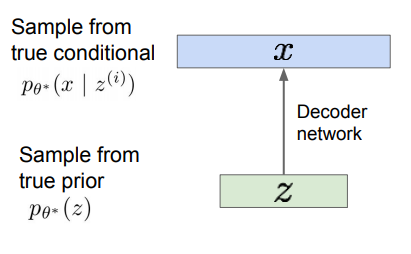
\includegraphics[width=0.33\textwidth]{img/vae_1.png}
\end{figure}

 We want to estimate the true parameters $\mathbf{\theta}^*$
of this generative model:

\begin{itemize}
    \item We choose the  prior ${p(z)}$ to be simple, e.g. Gaussian $p(z) \sim \mathcal{N}(0,\mathcal{I})$
    \item The conditional distribution $p(x|z)$ on the other hand is complex. We can model it with a neural network. In the case of images, an example would be a multivariate Bernoulli representing the state of each pixel $p(x|z) \sim Ber(\theta)$.
    \item We train the model to maximize the likelihood of the training data: $$p_{\theta}(x)= \int \overbrace{p_{\theta}(z)}^\text{Gaussian Prior}\overbrace{p_{\theta}(x|z)}^\text{Decoder NN}dz$$
\end{itemize}

However, the problem with this approach is that the \textbf{integral is intractable}: it is not feasible to compute $p(x|z)$ for every $z$.

\newpage
To overcome this,  we can define an additional encoder network $q_{\phi}(z|x)$ that approximates $p_{\theta}
(z|x)$ (note that $p_{\theta}(z|x)$ is intractable as well because of the integral computation).

\begin{figure}[h]
\centering
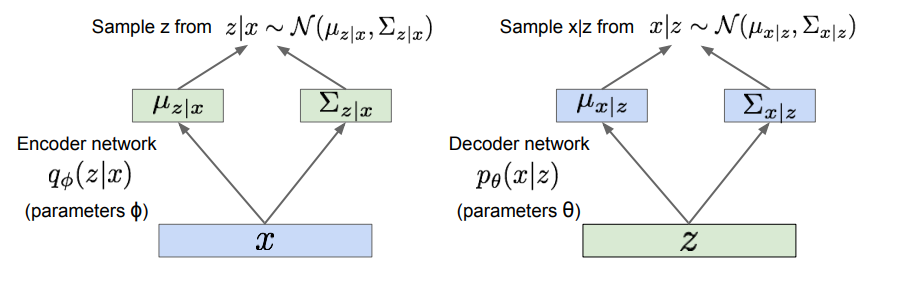
\includegraphics[width=0.8\textwidth]{img/vae_2.png}
\end{figure}


Now, we can find a lower bound (Evidence Lower Bound) for the likelihood of the training data:

\begin{equation*}
\begin{aligned}
   & \log{p_{\theta}(x^{(i)})} = \mathbb{E}_{z \sim q_{\phi}(z|x^{(i)}) } \Big[\log{p_{\theta}(x^{(i)})} \Big] &&&  (\text{$p_{\theta}(x^{(i)})$ does not depend on $z$})
   \\ & =  \mathbb{E}_{z} \Big[\log{\dfrac{p_{\theta}(x^{(i)} | z) p_{\theta}(z)}{p_{\theta}(z| x^{(i)})}} \Big] &&& \text{(Bayes Rule)} \\
   & =  \mathbb{E}_{z} \Big[\log{\dfrac{p_{\theta}(x^{(i)} | z) p_{\theta}(z)}{p_{\theta}(z| x^{(i)})} \dfrac{q_{\phi}(z|x^{(i)})}{q_{\phi}(z|x^{(i)})}}  \Big] &&& \text{(Multiply and divide by q)}
   \\ & =  \mathbb{E}_{z} \Big[\log{p_{\theta}(x^{(i)} | z)}  \Big] - \mathbb{E}_{z} \Big[\log{\dfrac{q_{\phi}(z|x^{(i)})}{p_{\theta}(z)}} \Big]  + \mathbb{E}_{z} \Big[\log{\dfrac{q_{\phi}(z|x^{(i)})}{p_{\theta}(z| x^{(i)})}} \Big] &&& \text{(Logarithms property)} \\
   & =  \overbrace{\mathbb{E}_{z} \Big[\log{p_{\theta}(x^{(i)} | z)}  \Big] - D_{KL}\Big(q_{\phi}(z|x^{(i)}) \; || \; p(z)\Big)}^\text{$=\mathcal{L}_{\theta,\phi}$ (ELBO)} + \overbrace{D_{KL}\Big(q_{\phi}(z|x^{(i)}) \; || \; p_{\theta}(z |x^{(i)})\Big)}^\text{$\geq 0$}
   \end{aligned}
\end{equation*}
In this context, the first term on the RHS  can be interpreted as expected negative reconstruction error. The second term is a regularization term that encourages the variational distribution to be close to the prior over latent variables. If the regularization term is omitted, the variational distribution would collapse to a delta function and the variational autoencoder would degenerate to a “usual” deterministic autoencoder.

Finally, we can find the optimal parameters optimizing the ELBO:

$$\theta^*, \phi^* = argmax_{\theta,\phi} \sum_{i=1}^{N} \mathcal{L}(x^{(i)},\theta,\phi)$$

\begin{figure}[h]
\centering
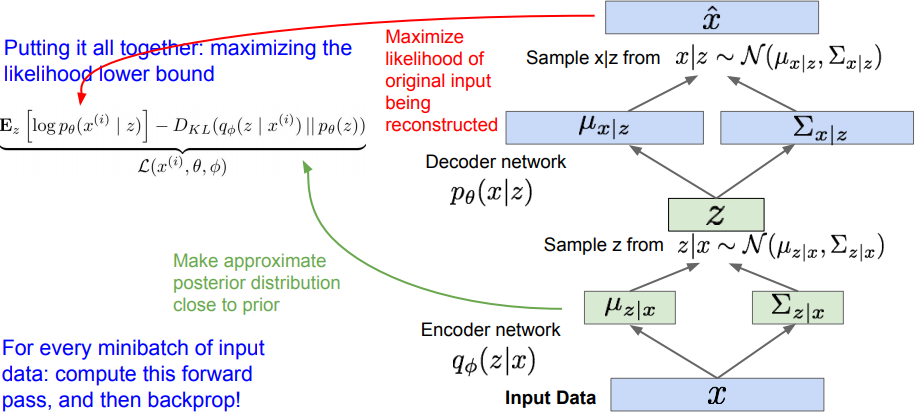
\includegraphics[width=0.45\textwidth]{img/vae_3.png}
\end{figure}

\end{document}
